\chapter{Attacks: what to expect}
\label{ch:attacks}
This chapter is about \textbf{attacks} and \textbf{what to expect} from an attacker. We will not see all possible attacks, but only some examples able to show the kind of stuff that we might come across in a network, and the consequences.

Attacks are always performed against a \textbf{vulnerability}: find a vulnerability, find an attack. Paradoxically, if we do not know that we have a vulnerability, attackers can do anything they want. Usually, if we are sure that we are not using a certain protocol/software/application (with certain known vulnerabilities), we can just ignore the attacks of that particular piece of software.
 
%----------------------------------------------------------------------------------------

\section{Classification}
Attacks can be classified according to the vulnerability or the layer they are leveraging, as follows:

\begin{itemize}
	\item application layer
	\item …
	\item transport layer
	\item network layer
	\item data link layer
	\item physical layer
\end{itemize}

Why the dots below the application layer? That area represents the Internet, and TCP/IP is not part of the ISO/OSI protocol. Normally, after the transport and network layer there are no other layers in Internet – although examples like the one below show that it is not always the case.

\vspace{0.5em}

\emph{Example} QUIC is a protocol invented by Google and later forwarded for standardization, where it has been heavily modified; it is used in HTTP3, a slight modification of HTTP2 which uses QUIC instead of TCP and TLS. QUIC runs on top of UDP, and provides all the session ideas on top it; basically, it reimplemented TCP on top of UDP. This, in practice, is an example of a layer located where the dots are in the previous layer list.

\vspace{0.5em}

%----------------------------------------------------------------------------------------

\section{Physical layer attacks}
There is not much to say about this kind of attacks, except that they are \textit{\textbf{phenomenally effective}} because they \textbf{disrupt the medium}. They go from network jamming (the most obvious) to the physical destruction of the network.

Physical layer attacks must never be underestimated. For example, jamming is very effective and the only way to stop it is to do a costly signal triangulation (i.e. find the emitting antenna, go there and physically kick the attacker’s ass). Physical layer attacks for wired networks are dangerous, too, because their probabilities of actually happening are not as slim as one might think:

\begin{itemize}
	\item in 2015 someone cut fiber optic cables in the Bay Area (California)\footnote{\url{https://www.wired.com/2015/11/security-news-this-week-bay-area-fiber-optic-cables-mysteriously-cut/}};
	\item in 2020 cell-towers have been attacked by idiots who claimed 5G spreads COVID-19\footnote{\url{https://arstechnica.com/tech-policy/2020/05/prepare-for-cell-tower-attacks-by-5g-covid-19-conspiracy-theorists-us-warns/}}.
\end{itemize}

Physical attacks have the additional advantage of being practically free, since the only thing needed is knowing where the cables are located. As for the network owner, they will probably have to replace a long cable, after having had an enormous area left without coverage (including ATMs, surveillance cameras, bank networks, etc.).

In order to prevent physical layer attacks we can use \textbf{redundancy}: we must not rely on a single physical element if we have a network that needs a high level of reliability.

\vspace{0.5em}

\emph{Example} Submarine fiber optic cables are very thick, even though they protect a cable as thin as a finger, because they have to be protected by sharks which gnaw on them. Seriously.

\vspace{0.5em}

%----------------------------------------------------------------------------------------

\section{Data link layer attacks}
\textbf{Data link layer attacks} are more sophisticated. They depend on the data layer protocol, so that attacks on Wi-Fi will not work on WiMAX, 802.15.4\footnote{IEEE 802.15.4 is a standard which defines the operation of low-rate wireless personal area networks (LR-WPANs). It is the basis for the Zigbee, ISA100.11a, WirelessHART, MiWi, 6LoWPAN, Thread and SNAP specifications.} or Ethernet.

\begin{itemize}
	\item \textbf{Wi-Fi RTS/CTS}: see section \ref{sec:wifi_rtc_cts_attacks};
	\item \textbf{packet flooding}: this kind of attack can be performed in almost all networks, as they consist in overflowing the network by sending too many packets;
	\item \textbf{datagram collision}: these are very effective and even simple, especially if there is some form of coordination in the network (e.g. in a token ring topology an attacker would simply have to generate a token in order to mess up with the whole system);
	\item \textbf{modifications to MAC-level timings}: in Ethernet, when the router is busy while someone is trying to send a packet, what happens if we have ten devices using one policy and another that uses a different policy to manage this situation? Chances are that either the one that disagrees is performing very badly, or that it is performing exceptionally well - meaning that the attacker is disrupting the network for the other users (because if it is using more resources than it should, the others will get less of them);
	\item \textbf{attacks to L2 devices}: even though they are quite difficult, there are many attacks of this kind (like the switch buffer overflow explained below), as the more complicated the system, the more creative is the attack.
	\begin{itemize}
		\item[] \emph{Example} L2 devices attacks like the switch buffer overflow leverage the fact that even if a system is stupid and does not have an operating system (like a normal switch), it still has some electronics and logic inside, because it has to decode packets and do forwarding after deciding the output port. What happens if two devices send two packets at the same time to the same device? This is where switches cost more or less: one will simulate a collision and drop both, another might hold one of the packets to send it later. The MAC-to-physical-port association table in a switch does not have the same number of entries as the number of physical ports on the switch, but many more (because for example we could have other switches on each port which multiply the number of inputs). If the switch does not have an entry in the table, it does not perform any kind of device discovery; instead, it simply sends the packet in broadcast to all ports. In doing so, though, it goes from being a full switch to being a hub, meaning that the performance of the system as a whole will drop (a lot). A normal user will notice an abrupt loss of performance, but will not know its reason (which could very well be an attacker).
	\end{itemize}
\end{itemize}
 
%----------------------------------------------------------------------------------------

\section{Layer 2.5 attacks}
\textbf{Layer 2.5 attacks} are a special case, as they are not really aimed at level 2.5 (which does not really exist), but target the APIs between L2 and L3 (the protocols necessary for gluing these two layers together, in particular the neighbor discovery protocol). Sometimes they are classified as MAC-level attacks, sometimes as layer 3 attacks.

Layer 2.5 attacks exist because in protocols like TCP/IP, where the data-link layer can be anything, we cannot make any assumptions about it, so we have to use some protocols able to perform stuff that L3 might not give for granted. These protocols are called \textbf{ARP} (\textbf{Address Resolution Protocol}, IPv4) and \textbf{NDP} (\textbf{Network Discovery Protocol}, IPv6), and they are both used for discovering the link layer address, such as a MAC address, associated with a given Internet layer address.

ARP and NDP are mandatory, because there is no other way to bind the IP address to a MAC address. Sometimes alternatives are used for NDP because of its high computational cost, but let us suppose that we use ARP and NDP only. In order to work correctly, they have the following requirements:

\begin{itemize}
	\item translate an IP address into a MAC address;
\item be plug \& play (have no need for configuration); this is the reason why there is no security or cryptographic key associated to ARP and NDP. They do have some \textit{“secured”} variants that ditch this requirement, but they are not really valid ideas because they are not effective (they need a key, which is a nightmare to distribute, and for security reasons they have to be periodically updated);
\item be fast (heavy protocols would be useless, since packets should take only a few milliseconds to transmit between devices);
\item support networks containing machines having variable IP addresses with respect to their MAC address;
\item support broadcast/multicast-enabled networks;
\item be able to quickly override an existing association (e.g. when swapping an Ethernet cable from one port to another, the device should retain its original IP address).
\end{itemize}

%-------------------------------------------

\subsection{ARP and NDP in a nutshell}
\textbf{ARP} and \textbf{NDP} work in the same way.

Our machines have buffers\footnote{Actually, there are buffers \textit{everywhere}.}. When sending a packet through IP, after having already passed through TCP or UDP, there is a thing called \textbf{ARP cache table} (IPv4), or \textbf{Network Discovery cache} (IPv6).

Each port has a buffer containing the IP and MAC addresses of all other devices attached to the same network, and their status (indicating if the entries are fresh). When sending a packet, the IP layer first checks if the IP address is in the table: if it is and it is fresh enough\footnote{ARP table entries can be \textit{valid}, \textit{stale} (old, but not completely invalid either, of the "hopefully it still works" kind), invalid and temporary (not yet configured). State transitions are as follows: \textit{temporary} $\Rightarrow$ \textit{valid} $\Rightarrow$ \textit{stale} (after some time) $\Rightarrow $ \textit{invalid} (stale for too long) $\Rightarrow $ \textit{deleted}; we can transition back from \textit{invalid} and \textit{deleted} with a valid request-reply exchange or a layer 4 message.}, the packet is sent immediately using the MAC address paired to that IP address.
 
Entries are generated and kept updated either by using L4 messages or ARP/NDP. In doing these exchanges, ARP and NDP are slightly different in the fact that NDP does not have a broadcast address (since it uses the solicited-node multicast address). Also, ARP does not use IP because the address frames are incapsulated directly in the Ethernet frame, while NDP uses ICMP, which is on top of IP: the main difference is that ARP has to maintain a lot of extra information, while NDP gets it directly from the ICMP and IP headers. 

%----------------------

\subsubsection{ARP datagram}
\begin{figure}[h]
    \centering
    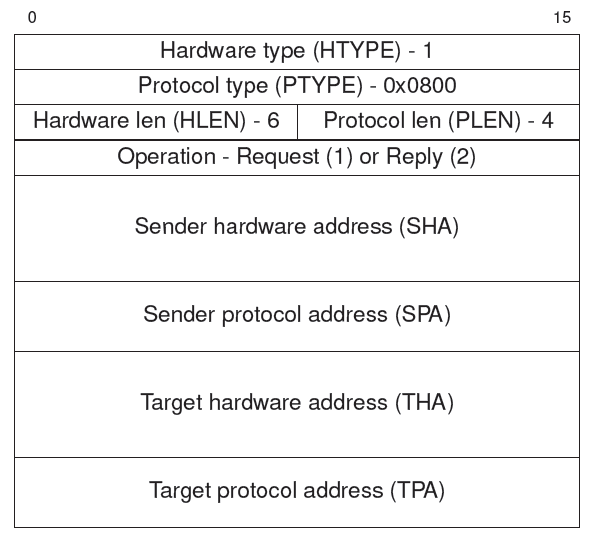
\includegraphics[scale=0.5]{img/arp_datagram.png}
    \decoRule
    \caption{Structure of an ARP datagram.}
    \label{fig:arp_datagram}
\end{figure}

The ARP frame is very simple. Some fields betray the fact that ARP has been foreseen to carry information of \textbf{any medium} and \textbf{any protocol} (not only Ethernet/Wi-Fi and IP). The fields are:

\begin{itemize}
	\item \textbf{hardware type} (HTYPE): equal to $1$ for Ethernet;
	\item \textbf{protocol type} (PTYPE): \texttt{0x0800} for IPv4;
	\item \textbf{hardware length} (HLEN): hardware address length in bytes ($=6$);
	\item \textbf{protocol length} (PLEN): IP address length in bytes ($=4$);
	\item \textbf{ARP operation}: can be either request ($=1$) or reply ($=2$);
	\item \textbf{sender hardware address} (SHA): usually the source MAC address;
	\item \textbf{sender protocol address} (SPA): usually the source IP address;
	\item \textbf{target hardware address} (THA): usually the destination MAC address;
	\item \textbf{target protocol address} (TPA): usually the destination IP address.
\end{itemize}

In this kind of datagram the request can be either sent in broadcast or in unicast. Usually broadcast is used when we do not know who the receiver is, so we send the packet to every node; unicast, on the other hand, is used whenever we have at least a good guess of where the destination is located (maybe we have an invalid or stale entry in the table and we send a unicast to try to recover it).

The reply can be either unicast or broadcast, too. The unicast reply is quite obvious: we send a broadcast request, and whoever wants to reply to it sends a reply only to us. The broadcast reply is called \textbf{gratuitous ARP}, and is not just useless, but the actual problem with the whole protocol.

Note that there is something missing in the frame, namely the \textbf{sequence number} (there is no way to pair a request and a reply, mostly because ARP does not care who is sending a reply and for what) and the \textbf{sender signature} (no protection against errors or spoofed addresses).

%----------------------

\subsubsection{NDP datagram}
\begin{figure}[h]
    \centering
    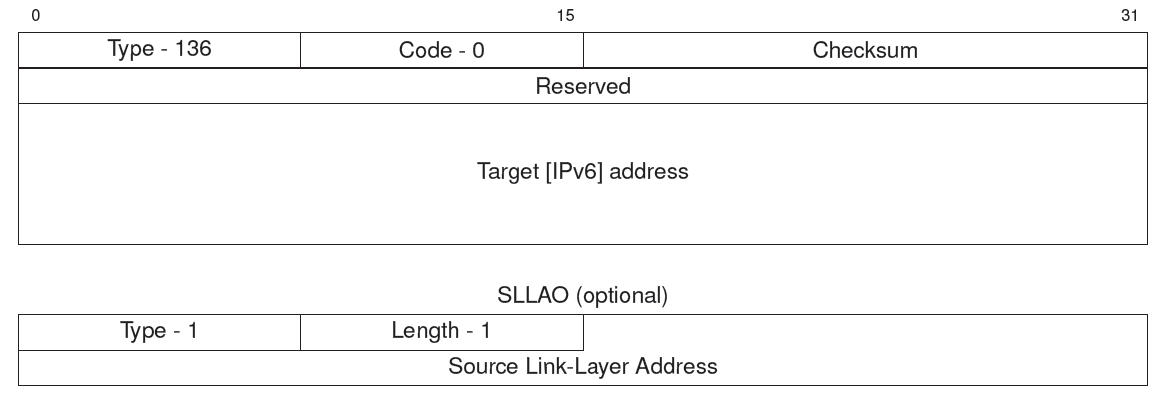
\includegraphics[scale=0.55]{img/ndp_datagram.png}
    \decoRule
    \caption{Structure of a NDP datagram.}
    \label{fig:ndp_datagram}
\end{figure}

The NDP frame is slightly different because it uses IP for its packets (ICMP messages are incapsulated in IP frames).

For this reason NDP does not need the sender’s IPv6 address, as it gets it from the IP header. The same goes for the source MAC address, which is carried by the MAC frame (this goes for ARP, too, where this address is actually redundant). However, if needed the source MAC address can be included in the SLLAO (Source Link-Layer Address Option): as a matter of fact, we can legally send NDP requests and replies at the same time from the same MAC address. The remaining fields are similar to those of the ARP frame.

The NDP reply is not identical to a request as it is in ARP, but is sent to the unicast address of the sender, and some bits are undefined so it is slightly shorter. The SLLAO contains the MAC address of the asker (in the request) and the replier (in the reply).

NDP is then a request-reply mechanism, where the request is sent to the solicited node multicast address and the reply to the unicast address (which does not need to be translated into a MAC address like in ARP, because it already is one and it is automatically translated directly into an Internet address at IP level). Usually, we receive a request, read the source link-layer address, create a temporary entry and send back a reply; if the sender sends another reply, then the entry is transitioned from temporary to valid. The reply is sent to the unicast address.

\vspace{0.5em}

\emph{Example} Let us suppose that we have two Ethernet cards with different MAC addresses, managed as a twin set; having two distinct MAC addresses is necessary because even if we had a perfect setup and managed to keep one of the NICs perfectly silent, the switch still would not have tables, so when we shut one down and bring the other one up this device would be confused because it would see the stuff from one cable on the other. In this case - which is definitely \textit{not} uncommon for enterprise-level systems - we want to instantaneously (or almost) switch the mapping of one IP address from a MAC address to another.

The problem here is that we have to inform whoever was talking to us that their ARP or NDP cache has to be updated, like, immediately, because if we do not do this there would be a short time, but still unacceptable in most cases, during which packets would get lost.

For example, suppose that Alice is talking to us, Bob; if we change our IP mapping, it will take some time before Alice realizes that she is talking to the wind, because she will assume that the packets are being dropped by the network for some random reason. Only when our ARP entry in Alice’s cache passes from valid to invalid she will send a unicast ARP request, and after seeing that failing she will (perhaps) use a broadcast, to which Bob will finally reply.

In the worst (normal) case the transition from a valid to an invalid or stale entry takes 30 seconds (timeout), during which Alice sends data but does not get any replies. The only way to inform her that something has changed is to proactively tell her that our address has been modified, which is where we send an unsolicited neighbor advertisement (gratuitous ARP).

\vspace{0.5em}

%----------------------

\subsubsection{ARP spoofing}
Let us consider an excerpt from \textbf{RFC 4861}:

\begin{quote}
    \centering
    \emph{\textbf{7.2.6. Sending Unsolicited Neighbor Advertisements}\\
In some cases, a node may be able to determine that its link-layer address has changed (e.g., hot-swap of an interface card) and may wish to inform its neighbors of the new link-layer address quickly. In such cases, a node MAY send up to \texttt{MAX\_NEIGHBOR\_ADVERTISEMENT} unsolicited Neighbor Advertisement messages to the all-nodes multicast address. These advertisements MUST be separated by at least \texttt{RetransTimer} seconds.}
\end{quote}

This passage contains an ambiguous sentence: \textit{“a node MAY send up to \texttt{MAX\_NEIGHBOR\_ADVERTISEMENT} unsolicited Neighbor Advertisement messages to the all-nodes multicast address”}. The standard is unclear: it does not say that we \textit{must} send it to the multicast address node, but only that we \textit{may} (or may not). So what happens is that it is not forbidden sending unsolicited neighbor advertisements to a unicast address, nor is forbidden for gratuitous ARPs to be sent to unicast addresses; as a matter of fact, this could be used as an optimization: referring to the example above, we would only inform Alice that our address has changed, and not everyone else's, too.

The only thing that we can do is to obey the regular request-reply order. The receiver will install a new entry in its ARP/NDP cache, which might be temporary or might refresh an old one, meaning that the last message to arrive wins. This is a requirement for failover cases\footnote{Failover is a procedure by which a system automatically transfers control to a duplicate system when it detects a fault or failure.}: we either do it like this, or we cannot perform failover techniques.

The obvious protection against unsolicited gratuitous ARPs is to add a sequence number: we do not accept replies if we did not ask for them. In doing so, though, we can forget about failover cases, which is something that we do not want to do.

But wait, why \textit{protection}?

Gratuitous ARPs are a vulnerability by design which allows the \textbf{ARP spoofing attack} (also called \textbf{ARP poisoning}). It goes without saying that this attack is valid for NDP, too.

\vspace{0.5em}

\emph{Example} Suppose we have three people: Alice, Bob and Eve, where Eve is an attacker unknown to the other two.

Eve sends a unicast gratuitous ARP to Alice claiming that Bob's IP address is reachable at Eve's MAC address, then does the same to Bob.

As long as Eve regularly sends these packets (every 30 seconds), Alice and Bob will have a valid transport layer connection flowing \textit{through Eve} (which has become a man-in-the-middle). The only thing that Eve must be careful about is making sure that the spoofed ARP/NDP caches of Alice and Bob remain valid, otherwise those two will send broadcast requests and will reply with the legit MAC addresses.

\vspace{0.5em}

The only caveat presented by this attack is that the attacker must be in the proximity of its victims (the same link-local network), since it is performed at link-local layer.

%----------------------

\subsubsection*{ARP spoofing countermeasures}

\begin{enumerate}
\item\textbf{Change the ARP/NDP protocol}: a short blanket kind of countermeasure, as it would certainly be effective in fighting the problem, but some requirements for this kind of protocol would inevitably be lost.

\vspace{0.5em}
	
\item \textbf{Check if someone is spoofing us}: every modern, decent system will ring a bell when seeing gratuitous ARPs claiming to be coming from ourselves; however, ARP/NDP messages can be sent using a unicast MAC address, and a switch will not send them to us, meaning that we will not be able to see them and raise an alarm.
	
\vspace{0.5em}
	
\item \textbf{Monitor the network for spoofed ARP/NDP replies}: the most used and effective method, it can only be implemented in the switch, which will block suspicious gratuitous ARPs and could still be configured to allow failovers from certain Ethernet cables.

\vspace{0.5em}

\item \textbf{Avoid letting the attacker in the local network} (fig. \ref{fig:meme_let_me_in_arp}): another very effective (and obvious) solution, which can be implemented by using the 802.1X AAA standard with a device configuration (basically, instead of authorizing users, it authorizes certain devices only (those presenting a given certificate), disallowing everyone else to send data on the cable they are attached to). Still ineffective against rogue interns.

\begin{figure}[h]
    \centering
    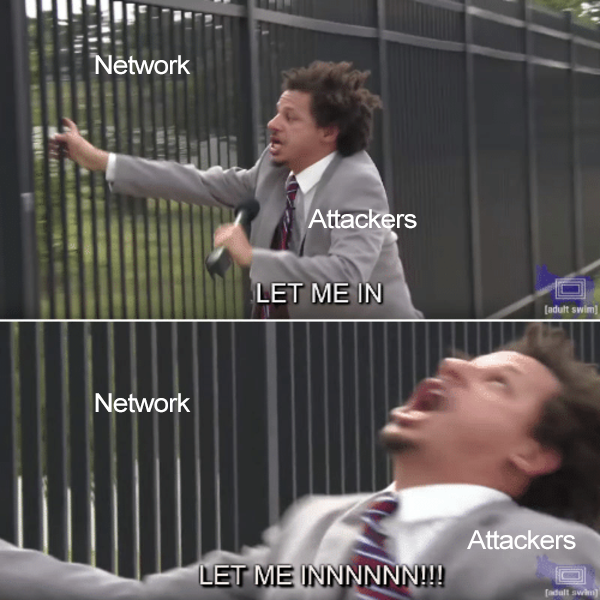
\includegraphics[scale=1]{img/meme_let_me_in_arp.png}
    \decoRule
    \caption{Even if they seem desperate, never let attackers in.}
    \label{fig:meme_let_me_in_arp}
\end{figure}

\end{enumerate}

%----------------------------------------------------------------------------------------

\section{Network layer attacks}
We will not enter into details about attacks on this layer because we would be discussing IP layer attacks, which do exist but are not relevant. Indeed, even though the IP layer does a lot of things, per se it is a simple mechanism with barebone functionalities and goals, and can only be leveraged for address spoofing and routing attacks\footnote{Routing attacks are, in fact, very dangerous, as they can subvert a network’s functionalities as they mess up with the packet’s destinations.}; it is mostly used as a basis for attacks on other specific protocols, which do not target the IP layer itself.

 %-------------------------------------------

\subsection{Fragmentation attacks}
The first attack we are going to discuss, as said, it does not target the IP (network) layer itself, but it uses its way of handling IPv4’s MTU in order to perform a \textbf{fragmentation attack}.

The \textbf{MTU}, or \textbf{Maximum Transmittable Unit}, is a fundamental requirement of the data link layer, as it specifies how long should a datagram’s payload be in a specific network segment.

Note that we must differentiate between \textbf{MTU} and \textbf{PMTU} (\textbf{path MTU}): the MTU is the one seen by a host on the network that it is attached to (so the host always knows what this value is), while the PTMU is valid along the whole path of the packet, from source to destination. Finding out the PMTU is not a simple task, as it cannot be known in advance; instead, the path must be probed first since in order to calculate this value the host needs to know the MTU of every network in between the source and the destination. What is worse, routing is not fixed, so the PMTU can still change during the actual transmission of a packet.

Fragmentation happens because the application layer of the source node gave to the transport layer a block of data that is too large for that network. This can happen for a number of reasons: for example, while TCP manages by itself how many bytes it transmits, UDP tries to feed all data in a single datagram, so it could very well give to the IP layer a large packet, and at that point IP would have to fragment it. A packet exceeding the MTU will be:

\begin{itemize}
	\item split between the IP and MAC layers (layer 2.5) and fragmented below the IP layer (an uncommon approach, but still employed by protocols like 6LoWPAN);
	\item dropped and trashed: a message will be sent the upper layers to notify them about this event, in the hopes that they will first split it before sending it again (this is how IPv6 handles them);
	\item fragmented by any router/host/device, like in IPv4.
\end{itemize}

The \textbf{IPv6} protocol simply has to know the host’s MTU; if an intermediate node gets a packet that will not fit in the next channel, it simply drops the packet and sends a message back telling the source what happened. This is because fragmentation is a responsibility of the source node in IPv6, which resorts to IP fragmentation only in extreme cases.

Vice versa, \textbf{IPv4} allows any router along the way to fragment a packet that exceeds the MTU of the next network, in a process supported directly by the IP header, which contains a fragment offset field used to pair different fragments of the same packet. The responsibility of rejoining fragmented packets falls to the final destination\footnote{Other protocols, like 6LowPAN, rejoin packets at the end of the network segment for which the fragmentation was needed (layer 2.5), allowing for a well-bounded fragmentation.}.

\begin{figure}[H]
    \centering
    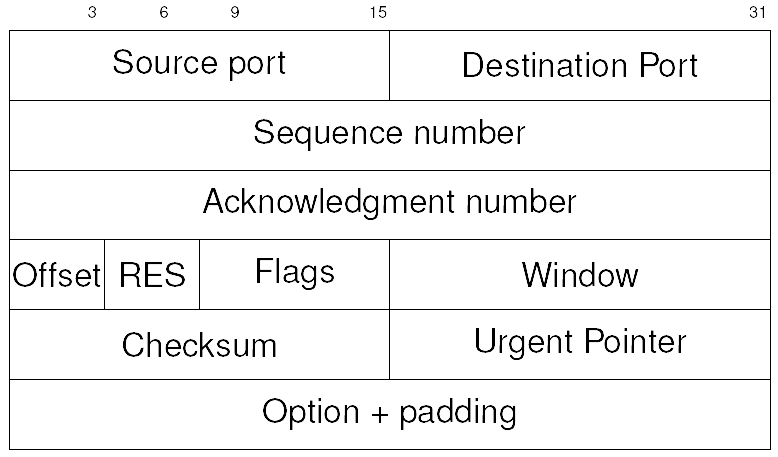
\includegraphics[scale=0.5]{img/tcp_header.png}
    \decoRule
    \caption{A simplified representation of the TCP header.}
    \label{fig:tcp_header}
\end{figure}
 
This approach poses a number of problems, mostly because of how the TCP header is made (fig. \ref{fig:tcp_header}) and how the fragment offset is calculated. Note that the flags in the TCP header contain the infamous SIN and ACK, the bits that tell if the packet is the start of a TCP connection or if it is part of a subsequent packet (these flags perform the three-way handshake).

\begin{figure}[h]
    \centering
    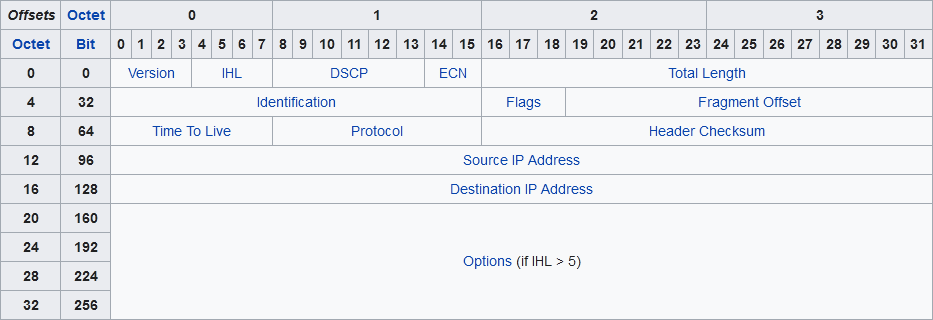
\includegraphics[scale=0.5]{img/ipv4_header.png}
    \decoRule
    \caption{Structure of the IPv4 header.}
    \label{fig:ipv4_header}
\end{figure}

Let us now examine the IPv4 header shown in figure \ref{fig:ipv4_header}: we can note that the \textbf{fragment offset} is measured in units of 8-byte blocks. But what is the \textit{minimum} size of a fragment? This value is given by the \texttt{1} in the fragment offset. An 8-byte block offset means that the first fragment of a packet carries data offsetted by 8 bytes with respect to the original one. If we check the TCP header in figure \ref{fig:tcp_header} we can see that an 8-byte block implies that the minimum first fragment contains only a source and a destination port, along with a sequence number - nothing more. This is an important (and questionable) fact, because at this point the TCP flags will be in the second fragment.

While this fragmentation process allows for a very high fragment granularity, it can easily be used for less orthodox employments.

A regular fragmentation would be expected to look like the one in figure \ref{fig:ipv4_fragments_expected}: every fragment has its IP header and some data about the original packet, and theoretically they would all be the same size (except for the last one, which could be shorter).

\begin{figure}[h]
    \centering
    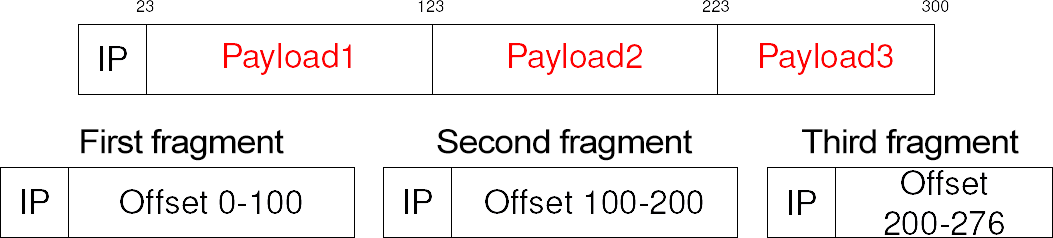
\includegraphics[scale=0.4]{img/ipv4_fragments_expected.png}
    \decoRule
    \caption{Expected IPv4 fragmentation of a packet.}
    \label{fig:ipv4_fragments_expected}
\end{figure}

However, if we create an extremely tiny first fragment, we can only squeeze it between the IP header and a very tiny part of the TCP header (the one containing the source and destination ports and the sequence number), as previously mentioned and now shown in figure \ref{fig:tiny_fragments_attack}. The acknowledgment, offset, fragment, checksum and other control flags will be in the second fragment, meaning that wherever a firewall is programmed to only allow packets \textit{not} containing a SYN flag, then that first tiny fragment (which does not have such a flag) will pass through. Chances are that the second fragment will pass, too, because even though it contains the SYN flag, it does not have a complete TCP header. In the end, we will completely bypass the firewall.

\begin{figure}[h]
    \centering
    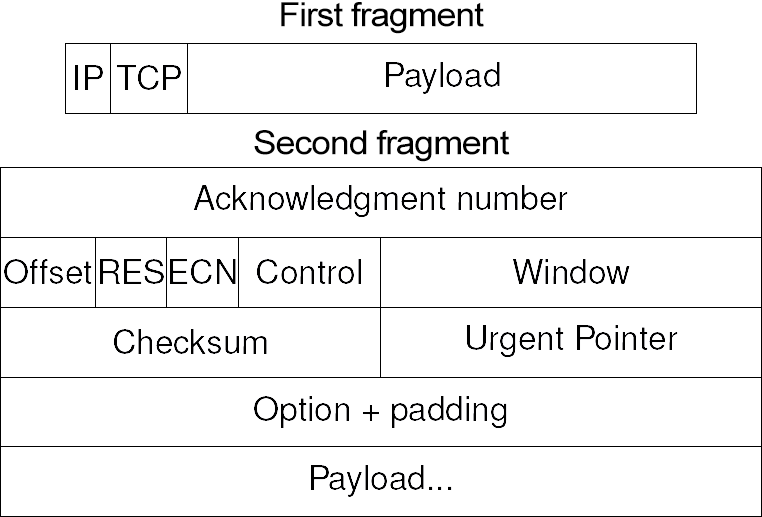
\includegraphics[scale=0.4]{img/tiny_fragments_attack.png}
    \decoRule
    \caption{Tiny fragments attack header structure.}
    \label{fig:tiny_fragments_attack}
\end{figure}

\textit{But wait, there's more.} We can do something even more creative. We can send the first fragment with a full TCP header and payload, and then \textbf{send a second fragment that overwrites part of the TCP header} itself (fig. \ref{fig:tcp_halves_meme}). This might look kind of illegal, but it is actually not - at least not in IPv4\footnote{IPv6 does not allow this procedure, so it normally does not suffer from this attack since it trusts the source node to only fragment a too large packet as needed, instead of adding extra/overlapping data, too.}.

IPv4 packets can be easily duplicated because of re-transmission. There is no guarantee that they will arrive, or that have been (not) reordered, or that they will arrive in a duplicated manner. Duplicated packets which travel along two different paths with two different MTUs might be \textbf{fragmented differently}; some fragments might get lost, while others might have been fragmented themselves into smaller parts. The end result is that overlapping fragments are totally legitimate.

In these cases one might think that the receiver checks what it has already received and fills in the holes. This might look like a reasonable approach, but in practice is highly inefficient, so what really happens is that at destination not only the missing parts are filled in, but already existing bytes are overwritten, too, without checking if the overlapping parts are actually identical. This mechanism allows for the so-called \textbf{IP fragmentation attack}, which is actually a TCP attack made using a feature of the network (IP) layer (more like a vulnerability by bad design).

\begin{figure}[h]
    \centering
    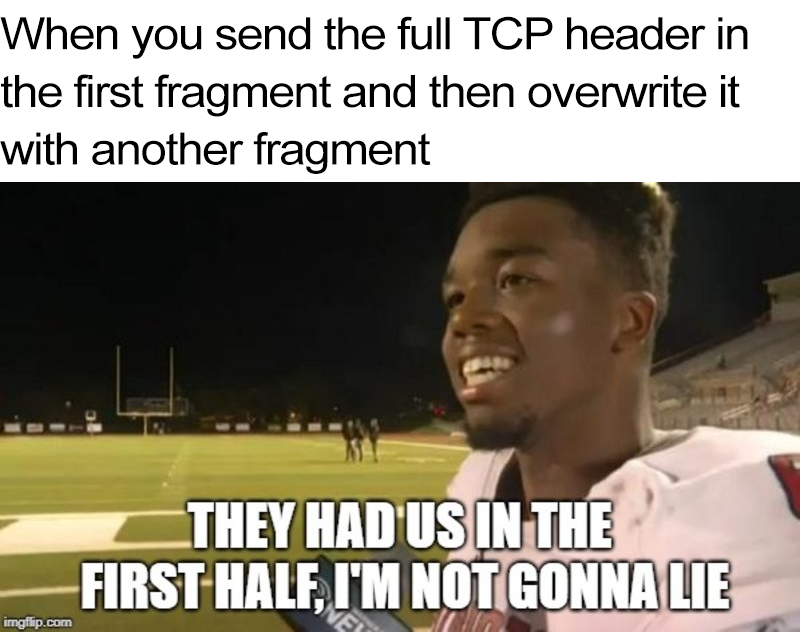
\includegraphics[scale=0.3]{img/tcp_halves_meme.png}
    \decoRule
    \caption{Overwriting headers is perfectly legit.}
    \label{fig:tcp_halves_meme}
\end{figure}

%----------------------

\subsubsection*{Countermeasures}
The simple, effective way to prevent fragmentation attacks is to deviate from the TCP/IP specification at its origin by rebuilding packets inside the firewall, so as to avoid bypassing it. Most firewalls nowadays work like this, although it requires additional resources on their part and leaves them vulnerable to \textbf{flooding attacks} made of a non-ending sequence of fragments which fills up their memory and makes them crash.
 
 %-------------------------------------------

\subsection{DNS attacks}
\textbf{DNS attacks} are another kind of attack which only partially involve the IP layer, since the DNS itself is an application level service.

The \textbf{Domain Name System} basically is the mechanism used to transform an alphanumeric string of characters in an IP address. It can be defined in many ways, but fundamentally it is nothing more than a huge, robust and redundant database. Its job is to receive a request (the IP address of a given alphanumeric address) and provide a reply (the set of IP addresses that respond to the given alphanumeric address).
 
A DNS attack aims at giving the user the wrong answer, possibly with the address of a website very similar to the requested one. If the user does not realize that they are visiting the wrong page, they might very well insert sensitive data, leading to \textbf{information leakage}.

\vspace{0.5em}

\emph{Example} A DNS attack is like going to the grocery store, asking for lemons and instead receiving limes: some people will notice that they are not the same and point it out, but others might not realize it and buy them anyway, maybe even thanking the store clerk for them.

\vspace{0.5em}

\begin{figure}[h]
    \centering
    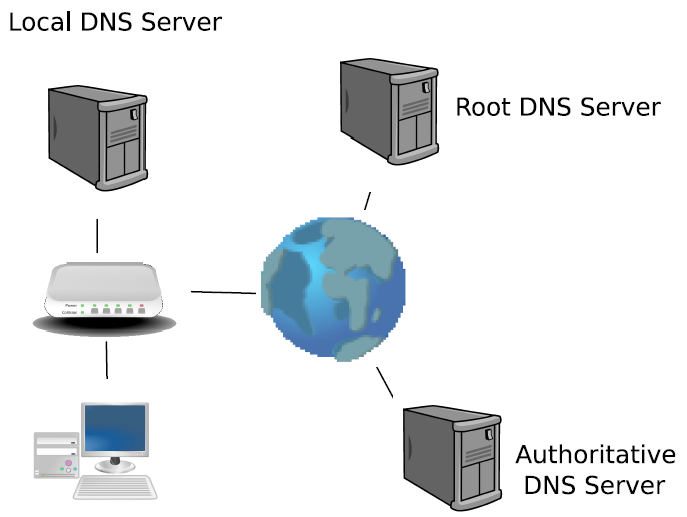
\includegraphics[scale=0.5]{img/dns_diagram.png}
    \decoRule
    \caption{DNS structure.}
    \label{fig:dns_diagram}
\end{figure}

The Domain Name System is made of three main elements, as shown in figure \ref{fig:dns_diagram}:

\begin{itemize}
	\item the \textbf{local DNS} server;
\item the \textbf{root DNS} server;
\item the \textbf{authoritative DNS} server.
\end{itemize}

Authoritative servers are specific to a group of addresses and are usually independently maintained by the organization who owns them.

\vspace{0.5em}

\emph{Example} The University of Florence hosts an authoritative DNS server that resolves all its addresses. A duplicated server is kept by the University of Bologna as backup.

\vspace{0.5em}

When asking for an address, the request goes to the local DNS server which, thanks to the tree hierarchy of the DNS servers, is able to reach the authoritative server and get a reply. Note that the reply is not sent directly to the host, but instead traverses the tree back to reach the local DNS server, which will then give the host the answer it is looking for.

\textbf{Caching} is employed in order to speed this process up. Caches have a validity time depending on when the record has been generated. However, a request for an authoritative server reply will skip the local cache and get a fresh reply (which in turn will be cached, refreshing an old entry). Before actually seeing how it is possible to trick the DNS into providing a wrong reply, let us see how it really works in practice.

A \textbf{DNS request} is performed through UDP. In order to pair requests and replies the following additional data is needed:

\begin{itemize}
	\item source IP address (the host’s for requests, the server’s for replies);
	\item source UDP port;
	\item destination IP address;
	\item destination UDP port;
	\item packet ID.
\end{itemize}

Let us focus on the reply. The source address of the DNS server that replied to us can be easily known. The same goes for the source UDP port, as it is always port 53. The destination IP address is also known. The only parts that - theoretically - should be unknown are the destination UDP port and the packet ID, so an attacker would only need those to perform an attack. Now, contrary to ARP, the DNS will trash any duplicate replies (which are legal since it uses UDP) instead of comparing them, meaning that the same attacker would have a super tiny window of time to send a spoofed packet (between the DNS request and the subsequent reply) - this does not, however, mean that such an attack is impossible outside the local path between the host and the local DNS server, as one might think.

First of all, let us see how to guess the right missing numbers from the UDP packet. If we would have to guess 32 bits right every time with a brute force approach, a DNS attack would not be possible because we would have to send 4 billion packets (about 160 GB of data) in an extremely short period of time. Unfortunately, some DNS servers do not use random ports for requests, but a single, random port, which can be reused once it has been guessed. This is \sout{crap} bad, but it is not enough: we would have to send about 5 MB of data in order to guess 16 bits, which are still too much for the given time frame.

Let us assume that the DNS request is not made by us, Alice, but by Bob, who is accomplice to Eve, an attacker. In this case Bob and Eve do not only know when the time window starts, but are also able to make it start whenever they want, allowing them to perform controlled random tries in order to guess the right DNS port.

The probability to match an ID by sending a random one is extremely low if we have only one shot at it (${\frac{1}{2}}^{16}$), but if we have a sequence of requests and we send a sequence of random guessed replies, the number of request-reply pairs needed to guess the correct answer drastically falls. By crunching some numbers we can find out that 700 tries have a probability of about 95\% to have a match, leading to the \textbf{poisoning} of the local DNS cache. The spoofed entry will remain there until it expires or somebody generates another authoritative server request (except that regular computers do not actually perform them).

The DNS attack is very common, and it can be applied not only to single addresses, but to whole domains. We can defend ourselves from them by making sure that the DNS request started from a random port, so the attacker will have to make $2^{32}$ tries.

We must also prevent him or her to trigger DNS requests on our local DNS server, meaning that we should accept DNS requests only from our trusted network (mind that this method does not work against insiders). \textbf{DNSSEC}, or Domain Name System Security Extension, is a valid alternative to DNS, as it provides cryptographically signed and cyphered communication between the local DNS server and the authoritative server.

\vspace{0.5em}

\emph{Example} Many (if not most) people use the Google DNS (\texttt{8.8.8.8} or \texttt{8.8.4.4}) or the one provided by Cloudflare (\texttt{1.1.1.1}). This means that these companies can track their users’ requests and know exactly what websites they are visiting (even in incognito mode, because requests always come with an IP address). And yes, they know how many times you visited \textit{that} website.

\vspace{0.5em} 

%----------------------------------------------------------------------------------------

\section{Transport layer attacks}

%-------------------------------------------

\subsection{SYN spoofing}
Sin, sin, everyone likes to sin. Like, we literally open connections every few minutes or so. Or was it \textit{SYN}? Whatever, you get it.

When a computer receives a SYN, it prepares for an incoming flow by reserving some memory for the TCP buffers.

A connection started by a SYN is sort of only half-open during the three-way handshake, but it still consumes resources - so what happens if we send a SYN but do not reply to the subsequent SYN-ACK? The simple answer is that the server trashes the SYN after a given timeout expires. The complicated one is that the timeout is \textit{critical}, as it is proportional to the \textbf{roundtrip time} (the one needed for a packet to go back and forth between the two devices performing the handshake), which cannot be measured since the SYN receiver does not know how much time the SYN took to get to it. In order to determine the timeout an assumption has to be made about the roundtrip time, and this assumption happens to be quite long and result in the holding of several megabytes of resources.
 
This attack is called \textbf{SYN spoofing} and consists of a \textbf{SYN flooding}: the attacker sends loads of SYN packets to a server, but does not answer to its SYN-ACKs. The interesting part about it is that the attacker does not even need to use its own IP address, as a spoofed one is sufficient and will have the SYN-ACKs go somewhere else (leaving the attacker’s bandwidth free). Once the attacker has taken up all the server’s resources with its own SYNs, the server will not be able to open new connections until the half-opened ones are gone.

As a countermeasure we can use \textbf{SYN cookies}, a variation which memorize little bits of information to pair a SYN with a possible incoming connection, but allocates the resources only when getting the last ACK. The SYN attack remains feasible, but extremely unlikely to happen.

%-------------------------------------------

\subsection{TCP reset guess}
A completely different attack at transport layer is the \textbf{TCP reset guess}, a very, \textit{very} bad design vulnerability made true starting with a simple question: how do we terminate a TCP connection?

TCP connections can be terminated either \textbf{ungracefully} or by sending a \textbf{reset flag}. TCP is a soft state machine, meaning that we need a constant flow of data in order to maintain the connection\footnote{Hard state machines are those which remain stuck in a certain state until receiving an explicit message to transition from it.}; if no replies are received in a given period of time, then the connection will be closed (ungracefully).

A reset flag, instead, indicates to the other party that the connection will be closed after having received it. And this kind of packet can be faked on an ongoing connection without even looking at the other packets in that flow.

As usual, an attacker needs to know:

\begin{itemize}
	\item source and destination IP addresses;
	\item source and destination TCP ports;
	\item the correct sequence number (inside the flow).
\end{itemize}

TCP ports can be guessed, while the sequence number only has to be \textit{decently} right: even though TCP is a flow-based protocol, packets at low level arrive in any order because of IP, so TCP considers right anything that fits in its receiving buffer. How large is this buffer?
 
The sequence number is 32 bits long, so we would need about 284 days to guess the right number (we would have to perform $2^{32}$ tries). However, TCP requires that a reset packet sequence number must fall within a 16 bit long window (which consists of the sequence numbers kept alive by the machine).

The result is that we need only 6 minutes to guess the right number with a 16k modem (which by the way is really slow), while a normal 45 Mb/s connection only requires about 13,6 seconds to 11 minutes in the worst case scenario (where we know nothing about the ports).

Nowadays TCP has the habit of using multipliers, shifting windows from $2^{16}$ to $2^{32}$ bits. Still, even if the TCP window is $2^{32}$ bits, we only have to make 4 guesses before getting the right number with a fast connection. Practically, we can easily use this attack to prevent our neighbor to watch Netflix or to kick our sister/coworker/friend out of the network.

The sequence number should have been at least 64 or 128 bit number, because even though the TCP window has been increased with the multiplier, this number is still bound inside the TCP header, which cannot be changed. For this reason, there is no way to prevent this kind of attack, not even by encrypting the connection (as the one thing that would need encryption is the TCP header itself).

%----------------------------------------------------------------------------------------
\section{Application layer attacks}
We move now to the application layer, above TCP. All attacks presented in this section are only a few examples of how much screwing can be done with bad implementations or design, because the actual number of attacks that are possible at this layer is much greater.
 
These attacks are extremely dangerous because they target what we use everyday, namely (and mostly) \textbf{web browsers}. They are slightly less dramatic than those that affect layers from TCP downwards, because it is always possible (well, less painful) to \textbf{change the upper layers}, so they can be mitigated by upgrading them.

%-------------------------------------------
\subsection{Input validation attacks}
Let us begin by showing the amount of damage made possible by simply developing with the brain shut off.

%----------------------
\subsubsection{SQL is love, SQL is life}
Since we are going to see how easy it is to not properly think about the consequences of what we are doing, we start with an extremely simple username and password HTML form:

\begin{verbatim}
<html>
    <form action=retrieve.php method="get">
        User: <input type="text" name="user">
        <br>
        Password: <input type="text" name="pass">
        <input type="submit" value="Login">
    </form>
</html>
\end{verbatim}

The corresponding PHP script is as follows:

\begin{verbatim}
<?php
    $link = mysql_connect(’localhost’, ’test’);
    mysql_select_db(’sql_inject’);
    $user = $_GET[’user’];
    $password = $_GET[’pass’];
    $result = mysql_query("SELECT secret FROM userdb WHERE user = ’$user’
        AND password = ’$password’");
    $row = mysql_fetch_assoc($result);
    
    echo $user."\’Secret is: ". $row[’secret’]. "\n";
?>
\end{verbatim}
 
Remember that PHP, generally speaking, is a really bad idea, and nobody is still using it nowadays (hopefully); it remains a good example of what can be done, though. Note that in this form the password is obfuscated for the user, but if we do not use HTTP with cryptography it will be transmitted in plain text - but we will ignore this matter for the moment, as it is not the most dangerous thing here. Also, the use of PHP is purely hypothetical in this example, because what we are really concerned with is MySQL.

\textbf{MySQL is an open-source relational database management system (RDBMS)}, or in our case the simplest way to handle a list of username-password pairs (although any other SQL database flavor would do).

SQL’s function in this script is to perform a query on the database and see if the inserted username and password are in there (hopefully \textit{not} stored in plaintext). If they have been retrieved, the server will present the user with some private data.

This process looks to be mostly bug-free, right? Wrong. It is actually highly bugged, and represents an excellent example of vulnerability by bad implementation (which can actually be found in a zillion websites in the wild).

\begin{table}[h]
    \centering
    \begin{tabular}{|c|c|c|}
        \hline
        \textbf{Username} & \textbf{Password} &\textbf{Secret} \\
        \hline
        Alice & 321 & 2131 \\
        Bob & 123 & 2sd1 \\
        … & … & …\\
        \hline
    \end{tabular}
        \decoRule
        \caption{An example of a simple SQL username-password table (called \texttt{userdb} in our PHP script).}
        \label{tab:sql_query}
\end{table}

An attacker who knows neither the username or password will not be able to retrieve the secret. As a general rule of thumb we should never tell a user which part of a query failed in case of wrong information (i.e. do not specify “user not found” or “password incorrect”), because it might give an attacker additional details which might help him or her to refine their attack.

The incriminating line in the PHP script is the SQL query, \texttt{SELECT secret FROM userdb WHERE user = ’\$user’ AND password = ’\$password’}, because the SQL engine interprets it exactly as it is since the PHP (or Python, Ruby, etc.) script simply substitutes \texttt{password} with whatever the user wrote. Practically, if we entered \texttt{'Alice'} and as a password we used a special character like the apostrophe (\texttt{‘}), the query would return an error, as the actual query would be \texttt{SELECT secret FROM userdb WHERE user = ’Alice’ AND password = ’‘’}. Clearly, if this error leaks to the user, he or she will know that the developer was as dumb as a pile of rocks, because at this point we can just modify the entry and instead of entering an apostrophe we can be more creative and use this vulnerability to get a user’s secret without knowing their password:

\begin{verbatim}
SELECT secret FROM userdb WHERE user = ’Alice’
    AND password = ’’ OR user = ’Alice’
\end{verbatim}
 
What is even worse is that in SQL there are many other special characters, like the minus (which indicates the beginning of a comment) which can be used to abusively get entire lines of a table, up to the point of dumping the \textit{entire database} without even knowing its structure. 

The lesson learned from this vulnerability does not, however, lie in the \textbf{SQL injection} by itself, but in the reason why it is actually possible.

In PHP 5 and successive versions the countermeasures are called \textit{magic quotes}, and consist of backslashed quotes that prevent a user from inserting them in a field and have them pass \textit{as is} to the backend. Nevertheless, the real problem lies in the fact that the developer did not check the input. As a matter of fact, SQL injection falls into the class of \textbf{input validation attacks}.

Input validation is damn painful ("and I will not tell you where it hurts the most"\footnote{Cit. prof. Pecorella.}), but we \textit{must always do it}, and not just when the user enters some text, but on every single function that we write.

%----------------------
\subsubsection{Cross-site scripting}
\textbf{Cross-site attacks} (\textbf{XSS}) are part of a broad class of attacks that can be performed whenever a website (or another similar application) presents the user with \textbf{third party provided} content.

These attacks are dangerous because their victims trust the websites they are visiting without realizing that some parts of them are actually provided by someone else, possibly even without using a secure (HTTPS) connection.

\vspace{0.5em}

\emph{Example} A simple echo HTML script has the following form:
\begin{verbatim}
<html>
    <form action=check.php method="get">
        Write something:
        <input type="text" name="string">
        <input type="submit" value="Ok">
    </form>
</html>
\end{verbatim}

And the associated PHP script that executes the echo is:

\begin{verbatim}
<?php
    $input = $_GET[’string’];
    echo "You wrote ".$input;
?>
\end{verbatim}

If we write some HTML text in the input, it will actually be executed when the page is rendered to the client. The text can be anything, from simple alerts to extra logins, popups and, more recently, even cryptominers: we can inject in the web page a simple script that mines cryptocurrency on the user's computer and gives us back the results (some websites have even made this into a public feature, using cryptocurrency mining instead of ads).

\vspace{0.5em}

It is clear from this example that the range of possibilities is pretty much limited only by our own imagination.

XSS attacks can be countermeasured, again, with proper input validation.

%-------------------------------------------
\subsection{Cookies}
\begin{quote}
    \centering
    \emph{This website uses cookies. By continuing, you agree to their use.}
\end{quote}

TCP is a connection oriented protocol. HTTP, per se, is REST (request-reply), and in its original form it did not need to send subsequent requests to previous requests because it was simply meant as a web crawling tool, and pages were not meant to be updated after downloading them.

Soon after its creation, however, it was clear that perhaps saving the current user’s state was necessary in order to avoid authorizing him or her for every single request they made to the server.

Since authorizations are at application layer, we could not rely on TCP and the fact that a session with the server was open, because it would be closed as soon as it stopped getting replies. Thus the W3C invented \textbf{cookies}, a hash value (mostly random) sent from the server to the client, stored by the latter and sent back to the server along with subsequent requests.

The browser blindly trusts cookies: if we give it the right cookie, it thinks that we are a certain user - no matter how we got that cookie, which is why cookies have an expiration time that is supposed to be short enough as to prevent an attacker from performing a brute force attack. To put it simply, if we are able to find the cookie, we skip the authentication process.

Now, dumping the cookies of a user is not a big deal. It is actually much worse if after doing this we send them to somebody else. Fortunately, nowadays cookies are not used for authentication and authorization anymore, but only for user tracking (yay).

%-------------------------------------------
\subsection{Ajax}
\textbf{Ajax} (\textbf{Asynchronous JavaScript and XML}) is a set of techniques using many web technologies on the client side to create asynchronous web applications. With AJAX, web applications can send and retrieve data from a server asynchronously (in the background) without interfering with the display and behavior of the existing page.
 
It represents another class of problems, and is representative of the “good idea gone wrong” or the “sounds good, doesn't work” categories. Ajax was recent around 2009, so nowadays it is considered to be old. We talk about it because it was one of the first technologies in its category, but JavaScript, HTML5 and a number of other things apply the same principles.

\begin{figure}[h]
    \centering
    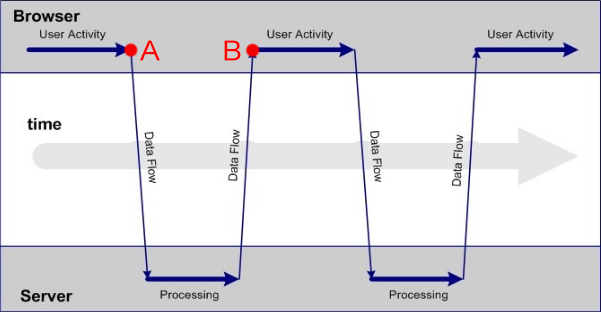
\includegraphics[scale=0.7]{img/webapp_model.png}
    \decoRule
    \caption{Classic web application model.}
    \label{fig:webapp_model}
\end{figure}

Ajax was conceived as a solution to the problem of developing a responsive application by hiding the delay between a normal client-server communication. Usually, when visiting a web page (or any other similar application), the client sends a command to the server and the server replies accordingly. Later, the user might send another command based on the server’s reply, resulting in a continuous flow of commands and replies. What happens is that from point A to point B (figure \ref{fig:webapp_model}) the client (user) sees the application as unresponsive, even in simple stuff like a drop down menu.

\begin{figure}[h]
    \centering
    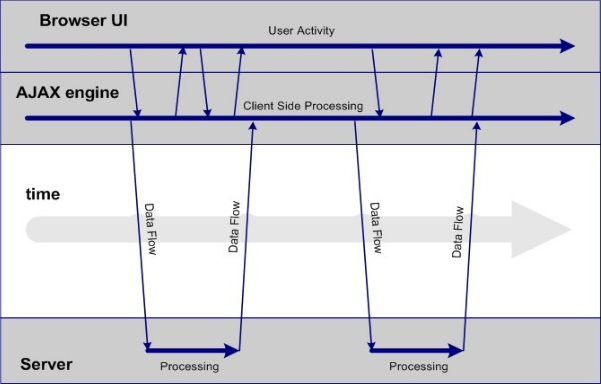
\includegraphics[scale=0.7]{img/ajax_app.png}
    \decoRule
    \caption{Ajax web application model.}
    \label{fig:ajax_app}
\end{figure}

This delay is very negative from the user’s point of view, and the only way to solve it is to transfer some processing from the server to the client.

The Ajax engine automatically transfers data to and from the server when necessary - which is not when the user clicks something (see figure \ref{fig:ajax_app}). When the application is written in a smart way, the user will see almost no delay in it. The downsides of this technology are that it is extremely dangerous (who would have guessed that?), for various reasons.

First, the controls for user login are not on the client side anymore, meaning that not only our application is caching somewhere our credentials, but also that the Ajax engine is storing them for a session, so we also have to trust the engine.

Second, communication and re-validation of the user also fall under the responsibilities of the engine (not of the application written by the developer), so in practice we lose control over sensible data.

For example, Ajax used to have a client side cache inside the engine, so if we wrote two different applications on the same engine nobody guaranteed us that the engine was sandboxing them correctly, and we could actually use its bugs to exfiltrate data. Nowadays this still happens in virtualization, so in general we can never trust a system to actually provide us with a perfectly trustable sandbox; we should not rely on sandboxing or caching at all.

\vspace{0.5em}

\emph{Example} Suppose that we wrote a set of libraries that allow us to embed an Excel table in Word, so that when we click on the table Excel opens, even if we are using Word’s interface. This is an example of an \textbf{embedded object}, a very bad idea which people periodically come up with.

\vspace{0.5em}

%-------------------------------------------
\subsection{Buffer overflow}
\textbf{Buffer overflows} are a problem that affects every programming language that allows us to write stuff in the computer memory - so basically everything. Any kind of buffer overflow allows \textbf{remote execution of arbitrary code}.

\vspace{0.5em}

\emph{Example} Let us consider the following C program:

\begin{verbatim}
#include <stdio.h>
#include <string.h>

int my_print_function(char*);

int main(int argc, char** argv){
    if (argv[1] != NULL)
        my_print_function(argv[1]);
    else
        printf("Nothing to print.\n");
}

int my_print_function(char* word){
    char text[10];
    strcpy(text, word);
    printf("The text to be printed is: %s\n", text);
}
\end{verbatim}
 
This program simply checks the input from the command line and prints it back: \texttt{argc} tells us how many parameters/variables/anything has been passed by the user in the command line, while \texttt{argv} contains a list of those values as null-terminated strings. Our system automatically breaks the latter down as a list, separating each block of stuff according to complex rules that include counting spaces, escape characters, double quotes, and so on.

In this case \texttt{argv} gets the first thing that we pass to the program and prints it back, or prints "Nothing to print." if the user did not input anything (it will contain a null/void value).

Checking if \texttt{argv[1]} is null is already a big mistake, as it only checks if a given memory location contains a value (if it does not, we will get the value of an uninitialized memory cell, which is very dangerous). We should actually see if \texttt{argc} has length 2 or more, for it is safer; note that when there are no parameters, \texttt{argc}’s length will still be equal to 1, as the first value is always the program’s name.

There is another mistake: in the function \texttt{my\_print\_function} there is an array called \texttt{text} which has a fixed value of 10 characters. The bug lies in the \texttt{strcpy} library function: this is a handy low-level function that copies a string from a pointer to another location, so from one area of memory to another area of memory, except that it blindly copies characters until it finds a termination of the source string (like the \texttt{0} character), so anything longer than 10 characters will be copied nonetheless.

If the input string is less than 10 characters \textit{including} the null termination, then everything will be fine. If it is longer, \texttt{strcpy} will keep writing stuff even after the reserved memory area, inevitably overwriting something else. If we are lucky, nothing will happen, and the program will actually work. If we are unlucky but still very lucky, the program will terminate, giving an error. If we are very unlucky, the program will seem to work, but it will actually do other things.

\begin{figure}[h]
    \centering
    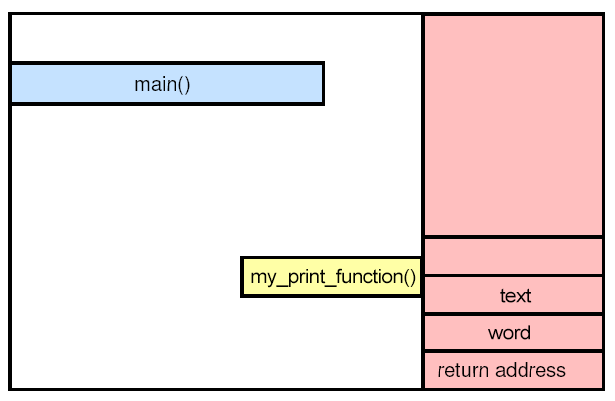
\includegraphics[scale=0.5]{img/buffer_overflow_example.png}
    \decoRule
    \caption{Memory structure of the above example C program.}
    \label{fig:buffer_overflow_example}
\end{figure}

\vspace{0.5em}

We can better understand this example by learning how data is laid out in memory. In there, a program is stored in two different areas, one for the program’s code and another for the stack (where temporary variables are stored). The stack has a dynamic scope, meaning that instead of being permanently reserved it is dynamically allocated when the function is called.

Besides the temporary variables, the stack also contains the return address, so if we are not careful we will overwrite it. Were this to happen, when the function terminates its execution the program will jump somewhere else in memory. This "somewhere" is \textit{not} the original point of the program that called the function, but any other location in the blank area. In C this memory space contains the whole standard library, which will start executing according to what it has found in the stack – the same stack wrote by us.

At the end of the day, a good programmer will be able to make the program do stuff like reading or writing files, writing other programs, or even executing a full, different program (\textbf{return-oriented programming wrap}). It can be demonstrated that in any sufficiently large program we can have a complete Turing machine just by using return-oriented programming, meaning that a simple program can be transformed in any other kind of program.
 
The simplest way to execute foreign code is to write a sequence of characters representing machine-executable code and then return to the stack itself. Even if the most common result will be a crash of the main application, an attacker has probably done his/her stuff in the meantime.
 
How can we protect ourselves from buffer overflows? First and foremost, we make our stack non-executable (plain simple), but we also must \textit{always} use functions like \texttt{strncpy}, the safe alternative to bugged library functions. And, most importantly: \textbf{we must always check the input}, be it from the user, a function, the command line or an external file. Other factors that can lead to a buffer overflow are:

\begin{itemize}
    \item \textbf{memory leaks}: they are extremely dangerous; under normal circumstances the program probably is not leaking, but usually the problem arises giving it an unexpected input;
    \item \textbf{temporary files}, beware of them: it is easy to write something on a file for some reason and then forget about it. Temporary files should thus not be trusted after a while because they might have been altered in the meantime (this is a form of information leakage);
    \item \textbf{system calls}: they should be considered by all means as untrustable (together with the whole operating system);
    \item \textbf{race conditions}, too, can lead to buffer overflows or other similar errors.
\end{itemize}

%-------------------------------------------
\subsection{Programming languages}
Programming language related issues are widespread. An example is the crazy \textbf{format bug} in C++, shown in the following example.

\vspace{0.5em}

\emph{Example} Let us return to the program from the buffer overflow example, this time using a version without the bugged \texttt{strcpy} function:

\begin{verbatim}
#include <stdio.h>
#include <string.h>

int my_print_function(char*);

int main(int argc, char** argv){
    if (argv[1] != NULL)
        printf(argv[1]);
    else
        printf("Nothing to print.");
    printf("\n");
}
\end{verbatim}

Here we check to see if \texttt{argv[1]} contains something, and eventually print it. How many bugs could be in here? Well... the \texttt{printf} function is the bug. \texttt{printf} actually is a multi-argument function, where the format and number of arguments are declared in the first parameter. Basically, \texttt{printf} reads the format string, finds the special symbols (beginning with \texttt{\%}), counts how many and what parameters follow, reads them from the stack and then replaces the \texttt{\%} with them before printing the string.

One would expect that the compiler will throw an error if the format of the first argument does not correspond to the subsequent variables (for example when trying to print \texttt{\%f} without having specified which number, \texttt{,x}). Usually, the compiler is smart enough to interpret the format string and understand that it was meant to have a second argument. But if the first argument (the format string) is something that we read on the fly, it cannot be analyzed, and this is where the bugs happen.

The user could write something like \texttt{\%x\%x}, which will not even throw an error at runtime, unless the programmer adds some exception check in the program - but still, it is risky: this input will make \texttt{printf} search for two values in the stack and print them as hexadecimal numbers.

If there is nothing on the stack and we try to retrieve something from it, those numbers will be whatever was in the stack before the \texttt{printf} function - and they can be used by an attacker. Basically we can achieve the very same effect of a buffer overflow with a single print. We should use the \texttt{cin} function instead, which is more robust (but also more picky and problematic when it comes to the format of the strings that are going to be printed, meaning that people will keep using \texttt{printf} because it is simpler).

\vspace{0.5em}
 
What can we learn from this? We have to fully master our programming language in order to provide the user with something that is decent enough - and when we say decent enough it is not because we are extra careful, but because for real we never know what is going to happen.

\vspace{0.5em}

\emph{Example} Another good example of vulnerability by library is that of the iOS \textbf{jailbreak}. Apple is a company particularly concerned with their application ecosystem: they only allow programs to run if they have passed through their own gates. However, this can be overcome with the so-called jailbreak. This technique used to be extremely difficult to perform until somebody found a bug in a library used by iOS to render PDFs. The end result was a webpage visitable from our iOS device: by simply loading it we would have started the jailbreak process.

\vspace{0.5em}